% Options for packages loaded elsewhere
\PassOptionsToPackage{unicode}{hyperref}
\PassOptionsToPackage{hyphens}{url}
%
\documentclass[
]{article}
\usepackage{lmodern}
\usepackage{amssymb,amsmath}
\usepackage{ifxetex,ifluatex}
\ifnum 0\ifxetex 1\fi\ifluatex 1\fi=0 % if pdftex
  \usepackage[T1]{fontenc}
  \usepackage[utf8]{inputenc}
  \usepackage{textcomp} % provide euro and other symbols
\else % if luatex or xetex
  \usepackage{unicode-math}
  \defaultfontfeatures{Scale=MatchLowercase}
  \defaultfontfeatures[\rmfamily]{Ligatures=TeX,Scale=1}
\fi
% Use upquote if available, for straight quotes in verbatim environments
\IfFileExists{upquote.sty}{\usepackage{upquote}}{}
\IfFileExists{microtype.sty}{% use microtype if available
  \usepackage[]{microtype}
  \UseMicrotypeSet[protrusion]{basicmath} % disable protrusion for tt fonts
}{}
\makeatletter
\@ifundefined{KOMAClassName}{% if non-KOMA class
  \IfFileExists{parskip.sty}{%
    \usepackage{parskip}
  }{% else
    \setlength{\parindent}{0pt}
    \setlength{\parskip}{6pt plus 2pt minus 1pt}}
}{% if KOMA class
  \KOMAoptions{parskip=half}}
\makeatother
\usepackage{xcolor}
\IfFileExists{xurl.sty}{\usepackage{xurl}}{} % add URL line breaks if available
\IfFileExists{bookmark.sty}{\usepackage{bookmark}}{\usepackage{hyperref}}
\hypersetup{
  pdftitle={GMACwriteup2.RMD},
  pdfauthor={Jarred Kvamme, University of Idaho},
  hidelinks,
  pdfcreator={LaTeX via pandoc}}
\urlstyle{same} % disable monospaced font for URLs
\usepackage[margin=1in]{geometry}
\usepackage{graphicx,grffile}
\makeatletter
\def\maxwidth{\ifdim\Gin@nat@width>\linewidth\linewidth\else\Gin@nat@width\fi}
\def\maxheight{\ifdim\Gin@nat@height>\textheight\textheight\else\Gin@nat@height\fi}
\makeatother
% Scale images if necessary, so that they will not overflow the page
% margins by default, and it is still possible to overwrite the defaults
% using explicit options in \includegraphics[width, height, ...]{}
\setkeys{Gin}{width=\maxwidth,height=\maxheight,keepaspectratio}
% Set default figure placement to htbp
\makeatletter
\def\fps@figure{htbp}
\makeatother
\setlength{\emergencystretch}{3em} % prevent overfull lines
\providecommand{\tightlist}{%
  \setlength{\itemsep}{0pt}\setlength{\parskip}{0pt}}
\setcounter{secnumdepth}{-\maxdimen} % remove section numbering

\title{GMACwriteup2.RMD}
\author{Jarred Kvamme, University of Idaho}
\date{9/22/2021}

\begin{document}
\maketitle

\begin{figure}
\centering
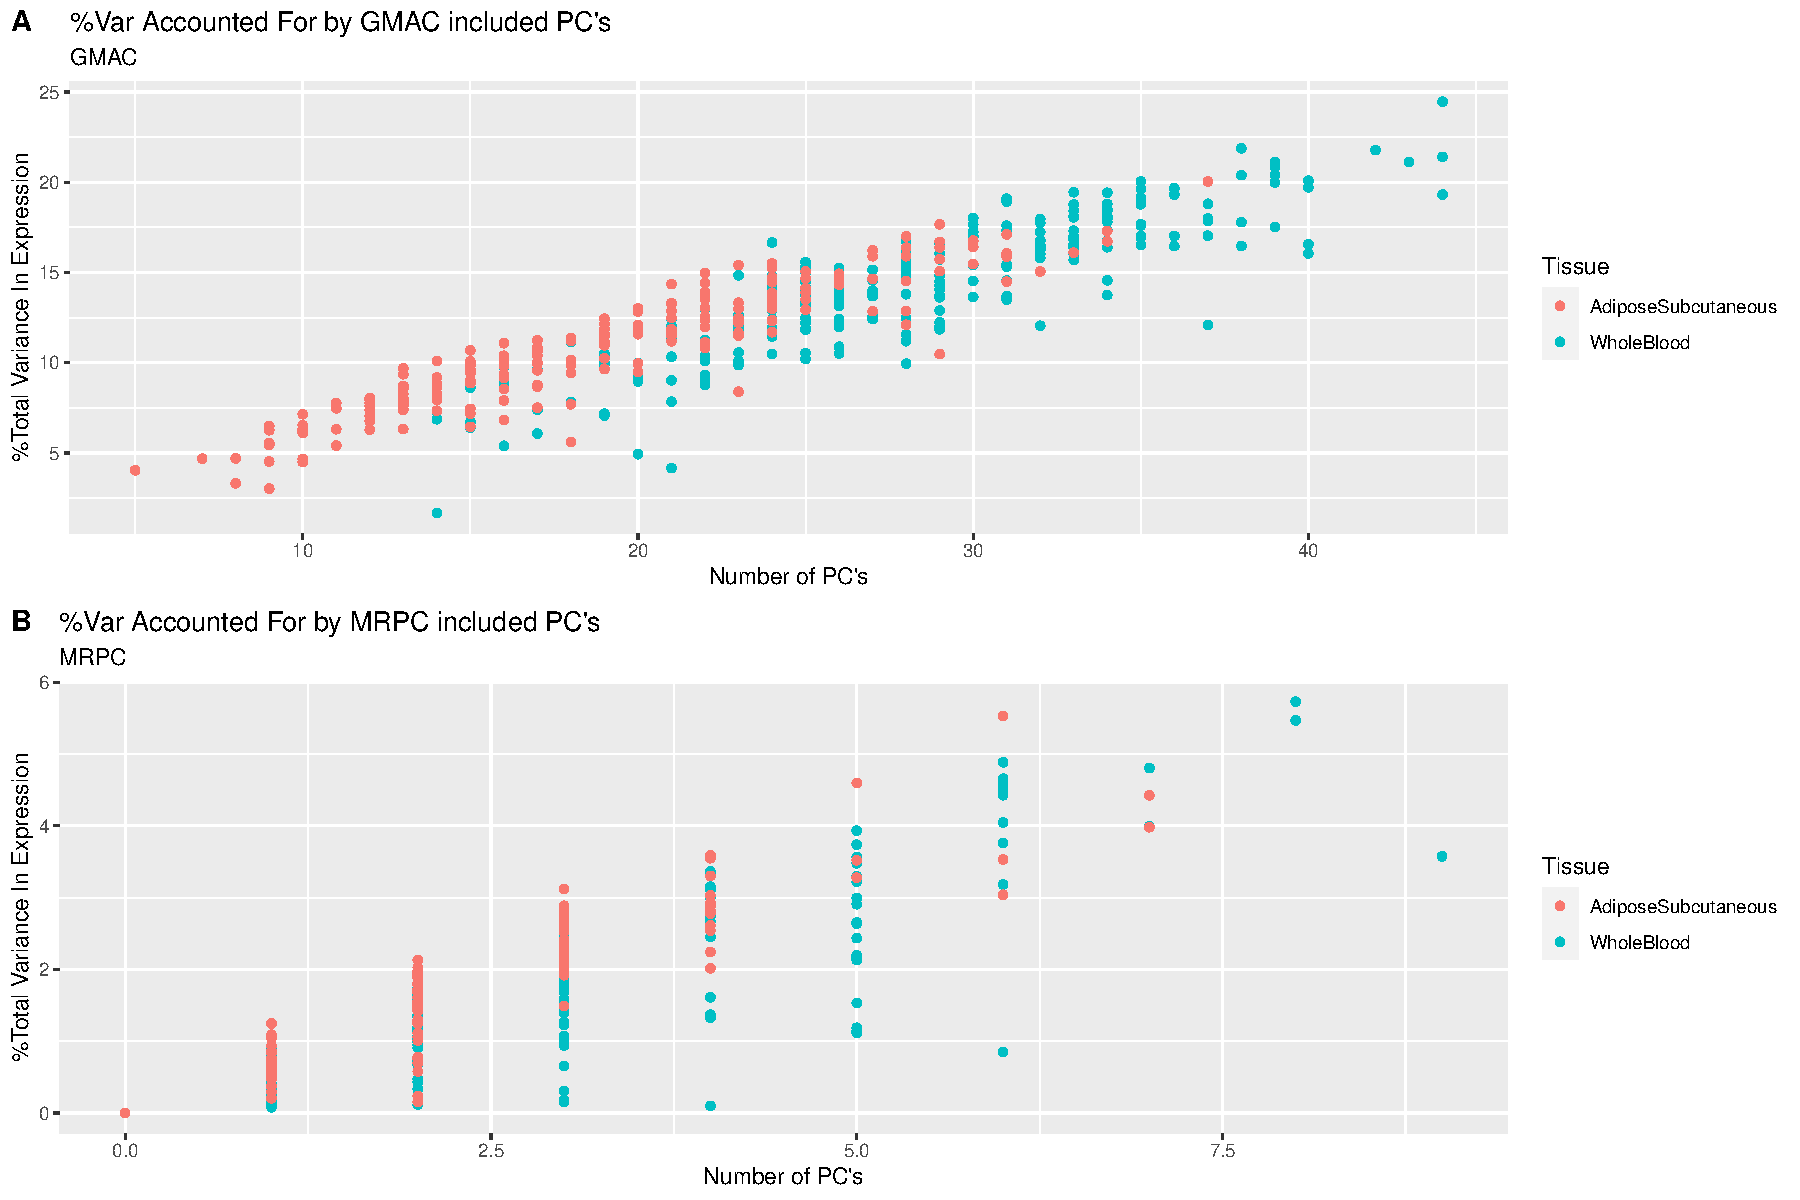
\includegraphics{GMACwriteup2_files/figure-latex/unnamed-chunk-1-1.pdf}
\caption{(A) scatter plots for the number of PC's included by GMAC and
MRPC (B) and the percentage of total variation in expression summarized
by the included PC's for each model}
\end{figure}

\begin{figure}
\centering
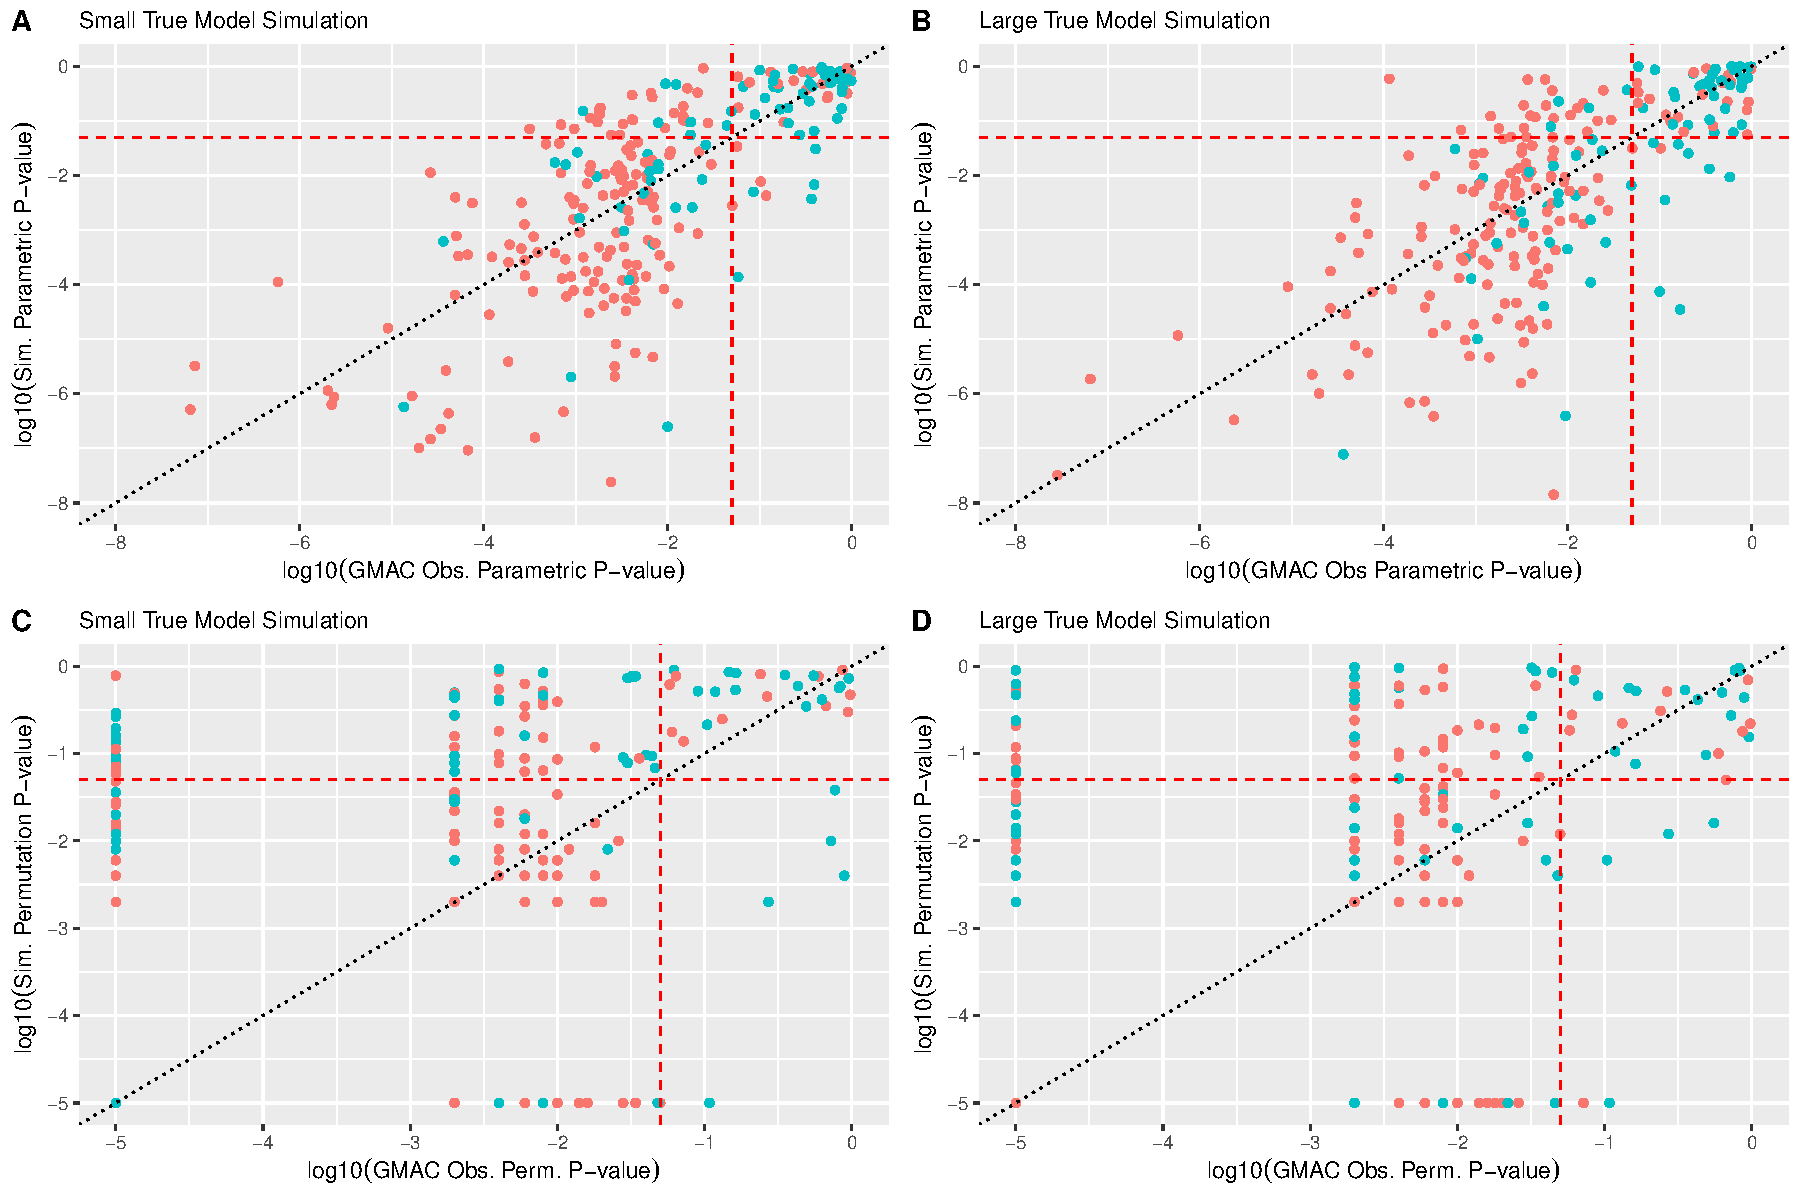
\includegraphics{GMACwriteup2_files/figure-latex/unnamed-chunk-2-1.pdf}
\caption{\textbf{(A)} and \textbf{(B)} the relationship between the
observed \(p\)-value of the mediation test and the \(p\)-value from the
simulated mediation test under the STM and LTM scenarios. \textbf{(C)}
and \textbf{(D)} the relationship between the observed \(p\)-value of
the permuted mediation test and the \(p\)-value from the simulated
mediation tests under the STM and LTM scenarios. In all plots blue
points represent trios with a rare allele observed at the SNP loci e.g
having a frequency among subjects below \(5\%\). The dotted lines define
the zone of insignificance at \(\log_{10}(\alpha) = -1.301\) scale. Note
that \(p\)-values \textless{} 2e-16 have been floored to \(2e-16\)}
\end{figure}

\begin{figure}
\centering
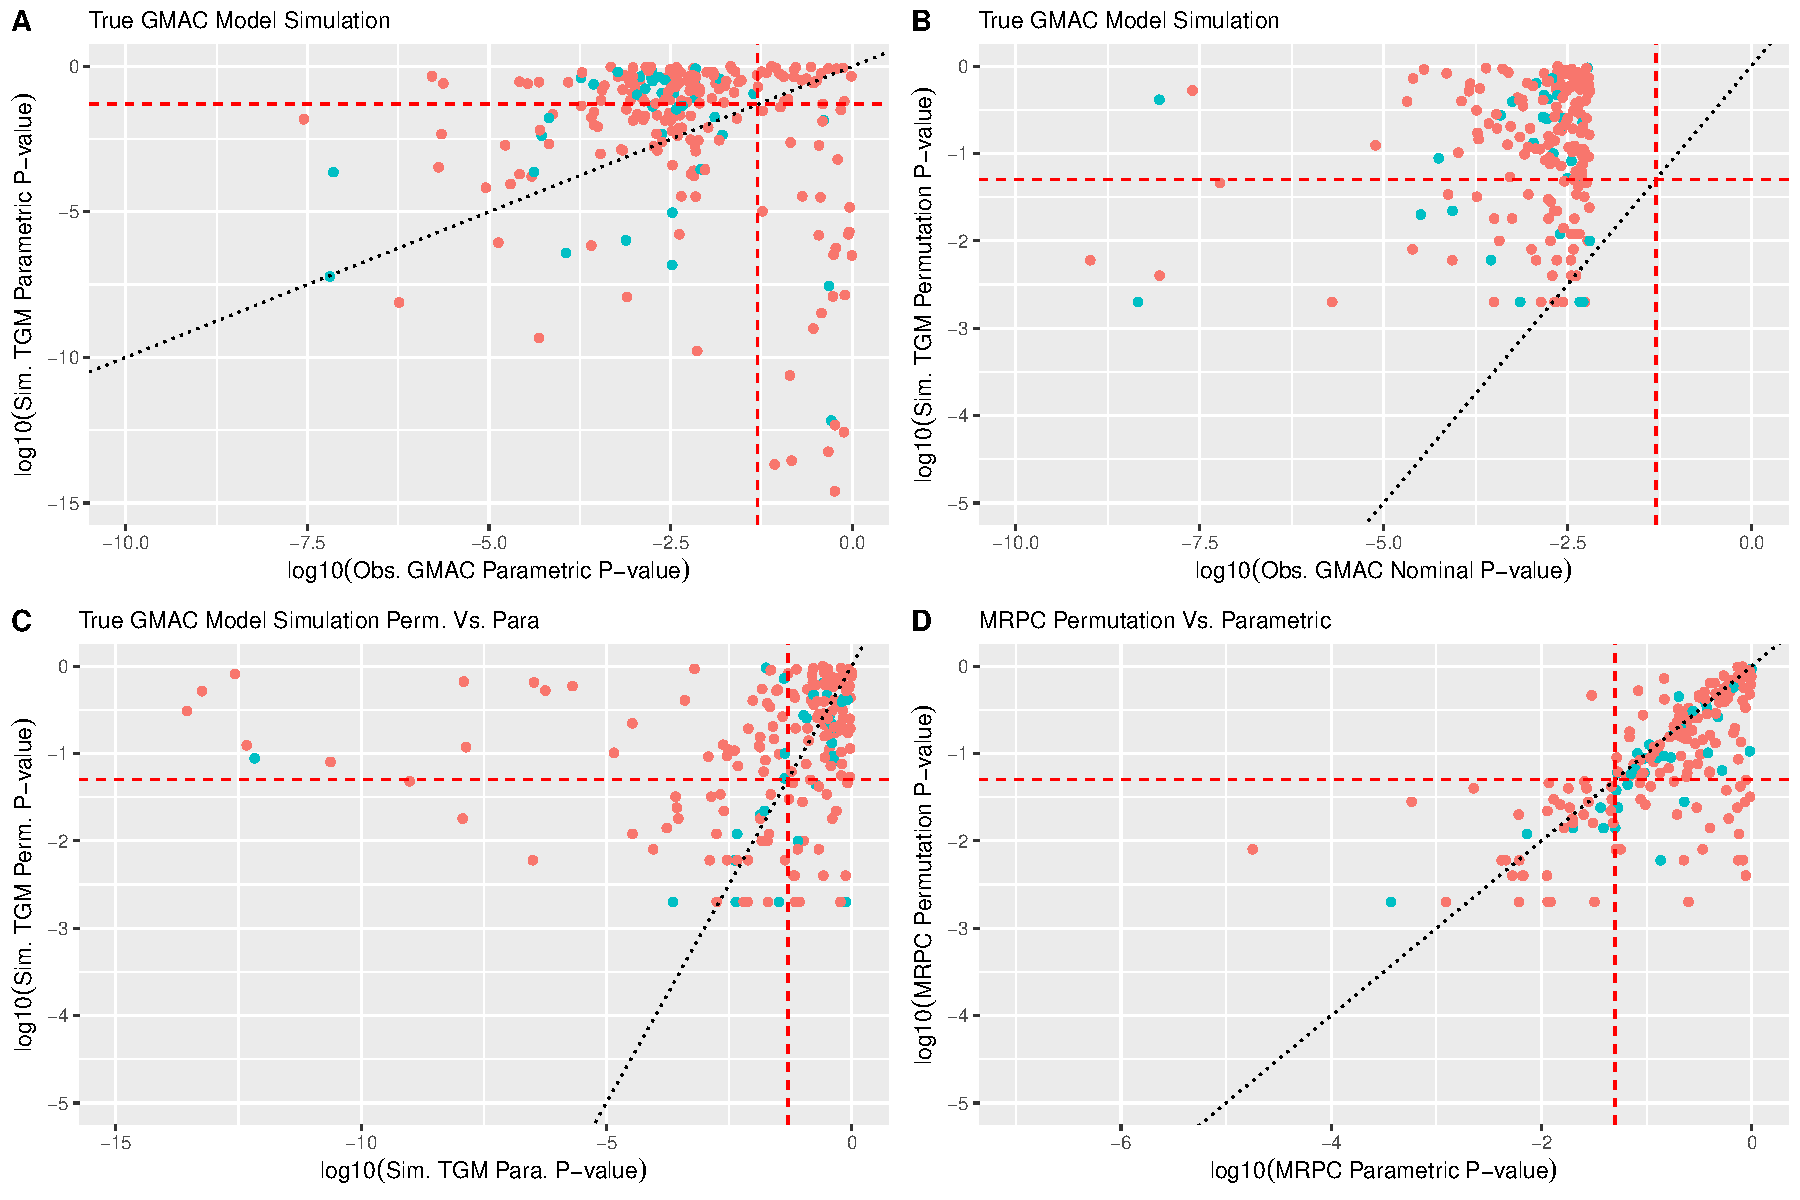
\includegraphics{GMACwriteup2_files/figure-latex/unnamed-chunk-3-1.pdf}
\caption{\textbf{A and B} Comparison of the observed parametric and
permuation \(p\)-values to those simulated under the True GMAC model
scenario. \textbf{C} comparison of the parametric to permuation
\(p\)-values withing the TGM simulation. \textbf{D} comparison of the
parametric and permuation \(p\)-values within MRPC}
\end{figure}

\begin{figure}
\centering
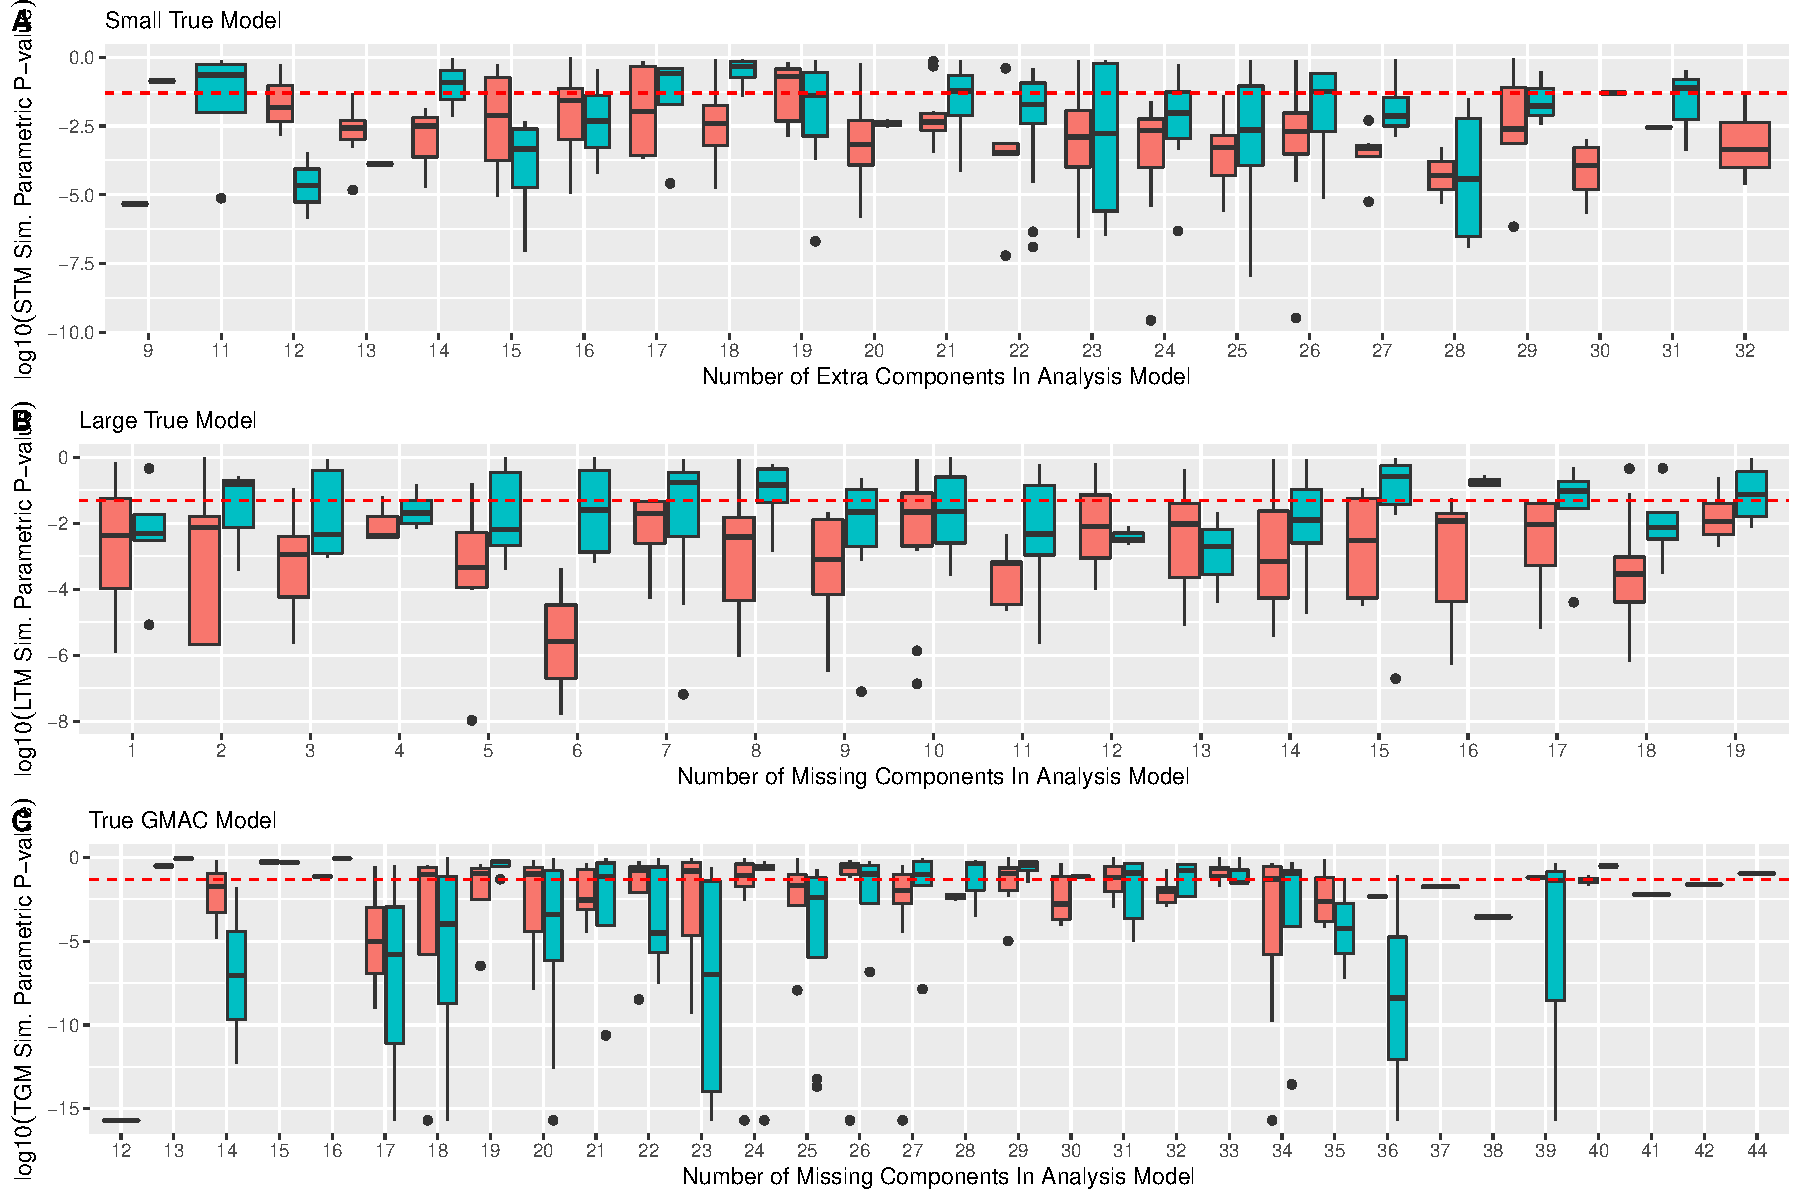
\includegraphics{GMACwriteup2_files/figure-latex/unnamed-chunk-4-1.pdf}
\caption{\textbf{(A)} and \textbf{(B)} The relationship between the
simulated mediation \(p\)-value and the number of additional (STM
scenario) or missing (LTM scenario) confounders in the analysis model
relative to the true model generating the trans gene. In both plots blue
boxes represent trios with a rare allele observed at the SNP loci e.g
having a frequency among subjects below \(5\%\).}
\end{figure}

\begin{figure}
\centering
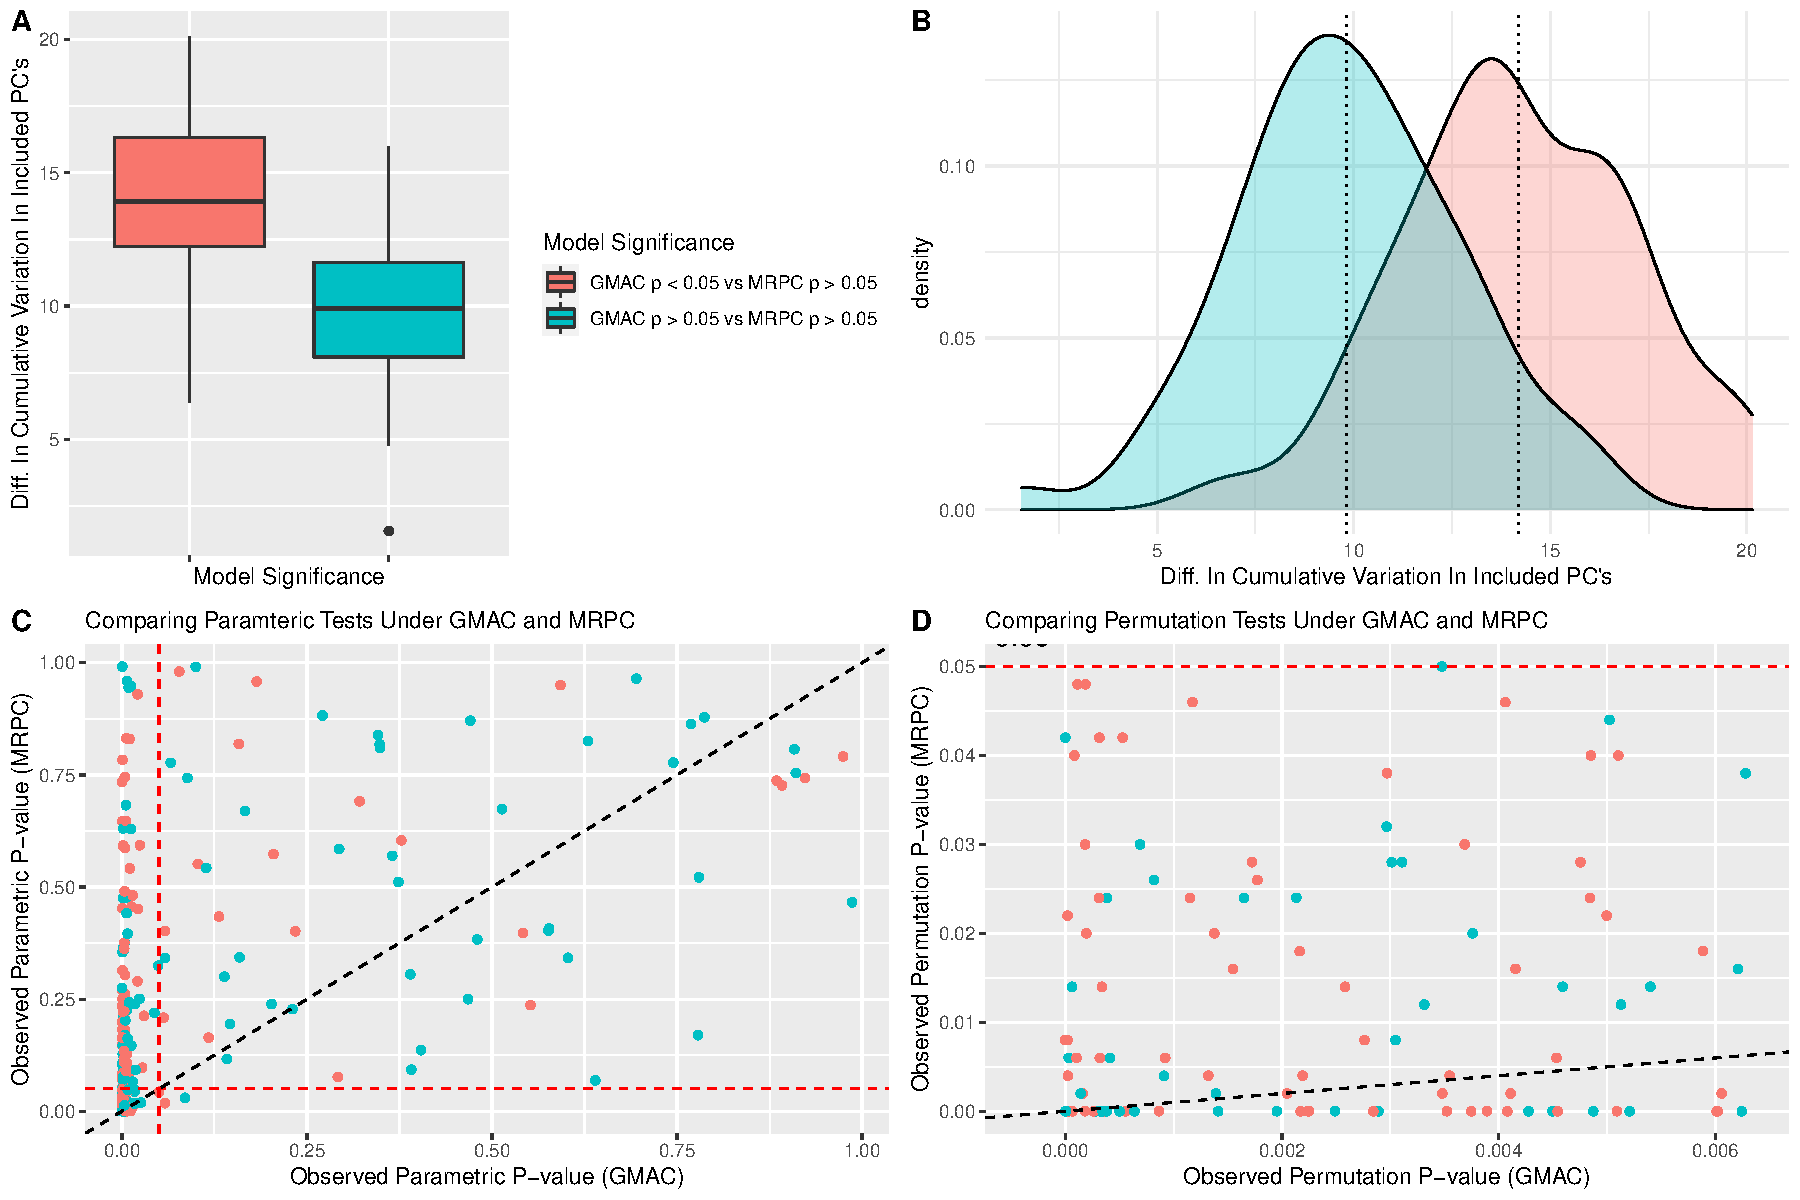
\includegraphics{GMACwriteup2_files/figure-latex/unnamed-chunk-5-1.pdf}
\caption{\textbf{A} The distribution of the difference between the GMAC
and MRPC models in terms of in percentage of variation captured by the
PCs/confounders included by each model, and under the special case of
trios for which the mediation test was significant under GMAC but
insignificant under MRPC \textbf{B} The distribution described for
\textbf{A} but under the alternative scenario when both GMAC and MRPC
mediation tests were insignificant (not to be confused with the
permutation test which is significant for GMAC). \textbf{C} Comparison
of the permutation and mediation \(p\)-values under GMAC. Blue points
indicate trios with a corresponding rare allele at the SNP loci.
\textbf{D} Comparison of the permutation and mediation \(p\)-values
under GMAC and excluding trios with a corresponding rare allele for
visibility. In \textbf{A,B,D} points along the black diagonal lines
indicate near \(1:1\) correspondence in the \(p\)-values between
methods.}
\end{figure}

\end{document}
